\documentclass[aspectratio=169]{beamer}
\usepackage{import}
\subimport{../../latex/}{setup_presentation}

\title{SYDE 750 Project}
\subtitle{Learning Probability Distributions for Statistical Inference}
\author{Andreas Stöckel}
\date{30th March, 2017}


\begin{document}

\maketitle

\begin{frame}{Lifespan Inference Task (I)}

Based on \emph{Optimal Predictions in Everyday Cognition} by Griffiths and Tenenbaum (2006)\\[0.5em]

\begin{columns}[t]
	\column{0.5\textwidth}
	\begin{itemize}
		\setlength{\fboxsep}{1pt}
		\item<1-> {\color{violet}Experimental task\textellipsis}\\[0.25em]
		\emph{Insurance agencies employ actuaries to make predictions about people’s lifespans---the age at which they will die---based upon demographic information. If you were assessing an insurance case for an \only<1>{18-year-old}\only<2->{\colorbox{violet}{\color{white}18-year-old}} man, what would you predict for \only<1>{his lifespan}\only<2->{\colorbox{violet}{\color{white}his lifespan}}?}
	\end{itemize}
	\column{0.5\textwidth}
	\begin{itemize}
		\item<2-> {\color{violet}\textellipsis as Bayesian inference}\\[0.25em]
		Given $t$, estimate $t_\mathrm{total}$
		\begin{align*}
			p(t_\mathrm{total} \mid t) = \frac{p(t \mid t_\mathrm{total}) \cdot p(t_\mathrm{total})}{p(t)} \,.
		\end{align*}
		Median estimator, select $\hat t_\mathrm{total}$ s.t.
		\begin{align*}
			p(t_\mathrm{total} > \hat t_\mathrm{total} \mid t) = p(t_\mathrm{total} < \hat t_\mathrm{total} \mid t) \,.
		\end{align*}
	\end{itemize}
\end{columns}
\end{frame}

\begin{frame}{Lifespan Inference Task (II)}

{\centering
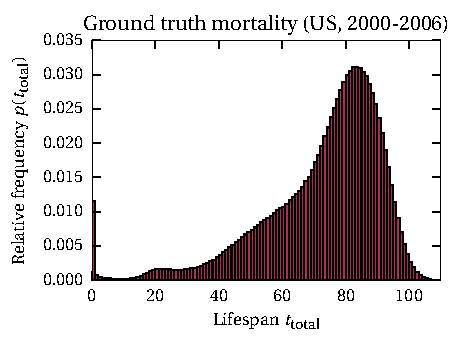
\includegraphics[scale=0.85]{media/mortality_ground_truth.pdf}
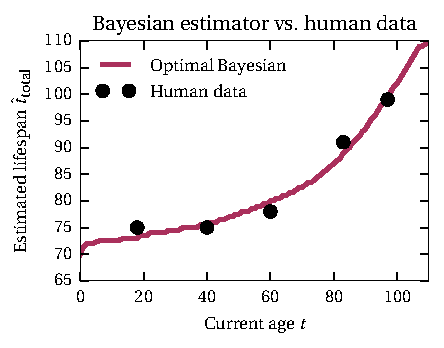
\includegraphics[scale=0.85]{media/mortality_optimal_bayesian_estimator.pdf}}

{\color{gray}\tiny \emph{Mortality data:} Human Mortality Database. University of California, Berkeley (USA), and Max Planck Institute for Demographic Research (Germany). Available at \url{www.mortality.org} (data downloaded on 2017/03/29). \emph{Human experiment results adapted from:} Optimal Predictions in Everyday Cognition. Griffiths and Tenenbaum (2006)}
\end{frame}

\begin{frame}{Learning Probability Distributions from Samples}

\begin{overlayarea}{\textwidth}{0.25\textheight}
\only<1-2>{
	{\color{violet}\emph{Goal:}} The longer a sample $x$ is presented, the larger $p(x)$ (without normalization).\\[1em]
	{\color{violet}\emph{Idea:}} Representation as a sum of basis functions $p(x) = \sum_i w_i \cdot \phi_i(x)$.% with $\langle \phi_i, \phi_j\rangle \approx 0 \: \forall i \neq j$.\\[1em]
}
\only<3>{
	{\color{violet}\emph{Cumulative distribution:}}
	\begin{align*}
		\int_{-\infty}^x p(x') \; \mathrm{d}x' = \sum_i w_i \cdot \int_{-\infty}^x \phi_i(x') \; \mathrm{d}x' = \sum_i w_i \cdot \Phi_i(x)
	\end{align*}
}
\only<4>{
	{\color{violet}\emph{Median estimation:}} Follow the gradient defined by
	\begin{align*}
		\int_{-\infty}^x p(x') \; \mathrm{d}x' - \int_{x}^\infty p(x') \; \mathrm{d}x' = \sum_i w_i \cdot \Phi'_i(x)
	\end{align*}
}
\end{overlayarea}

\centering
\includegraphics<1>{media/network_diagram_01.pdf}
\includegraphics<2>{media/network_diagram_02.pdf}
\includegraphics<3->{media/network_diagram_03.pdf}

\end{frame}

\begin{frame}{Implementing Lifespan Inference}

\begin{itemize}
	\item {\color{violet}Learning}\\[0.5em] Learn $p(t_\mathrm{total})$ by sampling from the ground truth, feed samples into the network\\[2em]
	\item {\color{violet}Lifespan estimation}\\[0.5em]
	Calculate above median-estimating cumulative function for the posterior
	\begin{align*}
		p(t_\mathrm{total} \mid t) &\propto p(t \mid t_\mathrm{total}) \cdot p(t_\mathrm{total}) &\text{where}\quad p(t \mid t_\mathrm{total}) &= \begin{cases}
			1 / t_\mathrm{total} & \text{if } 0 < t < t_\mathrm{total} \\
			0 & \text{otherwise}
		\end{cases}
	\end{align*}
	using a bivariate $\Phi_i(t_\mathrm{total}, t)$. Integrate the output to converge to the estimate.
\end{itemize}


\end{frame}


\end{document}
